\documentclass{article}
\usepackage{amsthm}
\usepackage{amsmath}
\usepackage{amssymb}
\usepackage{xcolor}
\usepackage{tcolorbox}
\usepackage{float}

% Define theorem styles
\newtheoremstyle{problemstyle}
  {\topsep} % Space above
  {\topsep} % Space below
  {\normalfont} % Body font
  {} % Indent amount
  {\bfseries\color{blue}} % Theorem head font
  {.} % Punctuation after theorem head
  {.5em} % Space after theorem head
  {} % Theorem head spec (can be left empty, meaning ‘normal’)
  
\newtheoremstyle{solutionstyle}
  {\topsep} % Space above
  {\topsep} % Space below
  {} % Body font
  {} % Indent amount
  {\bfseries\color{brown}} % Theorem head font
  {.} % Punctuation after theorem head
  {.5em} % Space after theorem head
  {} % Theorem head spec (can be left empty, meaning ‘normal’)

% Define problem and solution environments
\theoremstyle{problemstyle}
\newtheorem{problem}{Problem}[section]

\theoremstyle{solutionstyle}
\newtheorem*{solution}{Solution}

% Define problem types
\newcommand{\probtype}[2]{%
  \newcounter{#1}
  \setcounter{#1}{0}
  \newenvironment{#1}[1][]{%
    \stepcounter{#1}%
    \begin{tcolorbox}[colback=green!10!white,colframe=green!60!black,title={#2 \arabic{#1}\ifx\empty##1\relax\else: ##1\fi}]
  }{\end{tcolorbox}}
}

% Problem types
\probtype{N}{N}%Number Theory
\probtype{G}{G} %Geometry
\probtype{A}{A} %Algebra
\probtype{CB}{CB} %Combi
\probtype{CL}{CL} % Calc
\probtype{T}{T} % Trigo
\probtype{CG}{CG} % Coordinate
\probtype{STAT}{STAT} % Stat
\probtype{M}{M} % Misc

% Define idea environment
\newcounter{idea}[section]
\renewcommand{\theidea}{\thesection.\arabic{idea}}
\newenvironment{idea}{%
    \refstepcounter{idea}%
    \begin{tcolorbox}[colback=blue!10!white,colframe=blue!60!black,title={Idea \theidea}]
}{%
    \end{tcolorbox}
}
%commands
\newcommand{\dg}{^\circ}
\newcommand{\ii}{\item}
\begin{document}
\section{Key}
$\text{N1}\equiv$ Number Theory: Problem 1\\
$\text{G1}\equiv$ Geometry: Problem 1\\
$\text{A1}\equiv$ Algebra: Problem 1\\
$\text{CB1}\equiv$ Combinatorics: Problem 1\\
$\text{CL1}\equiv$ Calculus: Problem 1\\
$\text{T1}\equiv$ Trigonometry: Problem 1\\
$\text{CG1}\equiv$ Co-ordinate Geometry: Problem 1\\
$\text{STAT1}\equiv$ Statistics: Problem 1\\
$\text{M1}\equiv$ Miscellaneous: Problem 1\\
\section{Qustions Dump}
\begin{G}
Consider a circle of radius $6$. Let $B,C,D$ and $E$ be points on the circle such that $BD$ and $CE$, when extended, intersect at $A$. If $AD$ and $AE$ have length $5$ and $4$ respectively, and $DBC$ is a right angle, Find the length of $BC$
\end{G}
\begin{idea}
\textbf{Thales Theorem:}\\
If $A$, $B$, and $C$ are distinct points on a circle where the line $AC$ is a diameter, the angle $\angle ABC$ is a right angle.\\
The converse is also true, that is if $A$, $B$ and $C$ are distinct points on a circle and $\angle ABC = 90\dg$, then $AC$ is a diameter.\\
\end{idea}
\begin{idea}
\textbf{The Power of a Point Theorem} is a relationship that holds between the lengths of the line segments formed when two lines intersect a circle and each other.\\
There are three possibilities as displayed in the figures below.\\
\begin{itemize}
\ii The two lines are chords of the circle and intersect inside the circle (figure on the left). In this case, we have $AE\cdot CE = BE\cdot DE$.\\
\ii One of the lines is tangent to the circle while the other is a secant (middle figure). In this case, we have $AB^2 = BC\cdot BD$.\\
\ii Both lines are secants of the circle and intersect outside of it (figure on the right). In this case, we have $CB\cdot CA = CD\cdot CE.$\\
\end{itemize}
\begin{figure}[H]
    \centering
    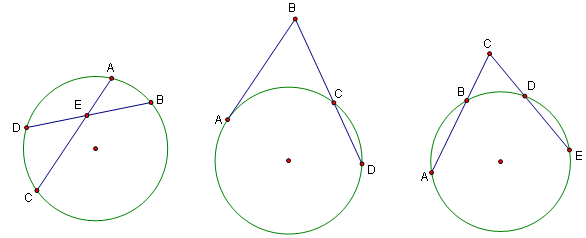
\includegraphics[width=0.75\linewidth]{images/Power of Point.png}
\end{figure}
The proof is using similar triangles.\\
\end{idea}
\begin{solution}
    Using Thales, $CD$ is a diameter. This means $\angle CED = 90 \dg$. This means $\angle DEA = 90 \dg$.\\
    In $\triangle{CED}$, we can use Pythagoras to get $EC^2+ED^2=DC^2 \implies EC^2+3^2=12^2 \implies EC=\sqrt{135}=3\sqrt{15}$\\
    We use power of a point to get $BA \cdot DA = AE \cdot AC \implies 5(BD+5)=4(4+3\sqrt{15})\implies BD = \frac{4(4+3\sqrt{15})}{5}-5 = \frac{12\sqrt{15}-9}{5}$\\
    Finally, we can use Pythagoras again to get $\boxed{BC=\frac{12+9 \sqrt{15}}{5}}$
\end{solution}
\begin{T}
    In a triangle $ABC$, the angle $BAC$ is a root of the equation $\sqrt3\cos x+ \sin x=\frac{1}{2}$ . Then the triangle $ABC$ is:\\
    (a) Acute angled\\
    (b) Righ angled\\
    (c) Obtuse angled\\
\end{T}
\begin{idea}
    We can use phasor method to convert sum of weighted $\sin$ waves to a single $\sin$ function. This method is detailed in physics(electricity, AC current related more accurately) texts normally.\\
    It can be described for this case as:\\
    $a\sin x + b\cos x = \sqrt{a^2+b^2} \sin (x+\arctan(\frac{b}{a}))$
\end{idea}
\begin{solution}
    Using the phasor method, $\sqrt{3}\cos x + \sin x = \sqrt{3+1} \sin(x+\arctan(\sqrt{3}))=2\sin(x+\frac{\pi}{3})$.\\
    This implies $2\sin(x+\frac{\pi}{3}) = \frac{1}{2} \implies \sin(x+60\dg)=\frac{1}{4}$\\
    As angles of a triangle are are between $0\dg - 180\dg$, and as $\sin$ is increasing from $0\dg$ to $90\dg$ and decreasing till $180 \dg$\\
    We can hence eliminate the value close to $0\dg$ as subtracting $60\dg$ will give a negetive angle.\\
    The angle closer to $180\dg$ will still be greater than $150\dg$ as $\sin(150 \dg)=\frac{1}{2}$. This implies the subtracting $60 \dg$ will still keep it above $90 \dg$. Hence, the triangle is obtuse angled.\\
\end{solution}
\begin{CL}
If $0<x<1$ and
$A_n=\frac{x}{1-x^2}+\frac{x^2}{1-x^4}+....+\frac{x^{2^n}}{1-x^{2^{n+1}}}$ then $\lim_{n\to\infty}A_n$ is ?
\end{CL}
\begin{idea}
    \[a+ar+ar^2+ar^3+\dots=\frac{a}{1-r}\]
    for $|r|<1$\\
\end{idea}
\begin{solution}
Using the infinite GP sum, we have $\frac{x}{1-x^2}=x+x^3+\dots=\{x^{2n+1}\}$\\
Similarly, $\frac{x^2}{1-x^4}=x^2+x^6+\dots=\{x^{4n+2}\}$\\
The sum can therefore be written down as $\{x^{2n+1}\}+\{x^{4n+2}\}+\dots= \{x^{2^{m+1}n+x^m}\}$\\
We claim that every number appears in this sequence only once. We can prove that no two sequences have any numbers in common by simple algebra. With infiinite sets with no reperting members, we cover infinite numbers.\\
Hence, $\lim_{n\to\infty}A_n = x+x^2+x^3+\dots = \frac{x}{1-x}$
\end{solution}
\begin{CB}
    A rabbit hops up a 7-step staircase. In each hop the rabbit can climb either one step or two steps. What is the no of different ways in which the rabbit can go upstairs?(The order of hops matters.)
\end{CB}
\begin{solution}
    Let's say that the rabbit covers $n$ steps in $H_n$ ways. The last step could either be one step hop or a two step hop.\\
    If it was a one step hop, we could have reached that point by $H_{n-1}$ ways. If it was a two step hop, we could have reached that point in $H_{n-2}$ ways.\\
    This means $H_n=H_{n-1}+H_{n-2}$. We know the value by direct computation for $H_1=1$ and $H_2=2$. We can simply calculate till $H_7=21$.\\
\end{solution}
\begin{CB}
    In how many ways can you choose three distinct numbers from the set $\{1,2,....,20\}$ such that there product is divisible by $4$?
\end{CB}
\begin{solution}
The Possible cases are:
\begin{itemize}
\ii Two even one odd
\ii Three even
\ii Two odd and one is a multiple of $4$
\end{itemize}
So,total number of ways $=\binom{10}{2}.\binom{10}{1}+\binom{10}{3}+\binom{5}{1}.\binom{10}{2}=795$
\end{solution}
\begin{N}
    Let $a_1=2$ and for all natural no n, define $a_{n+1}=a_n(a_n+1)$. Then , as $n\to \inf$ , the no of prime factors of$a_n$=?
\end{N}
\begin{solution}
    Note that $a_{n+1}$ has more prime factors than $a_n$. We can prove this using the facts that $x, x+1$ are coprime(share no factors) and that a number is either prime or has prime factors.\\
    As $a_{n+1}=a_n(a_n+1)$, $a_{n+1}$ has all the factors of $a_n$ and $a_n+1$. As $a_n$ and $a_n+1$ share no common factors, all factors of $a_n+1$ are present in $a_{n+1}$ but not in $a_{n}$.\\
    This means we are asking the endpoint of an monotonically increasing sequence, which is no of prime factors of$a_n$. We know this to be $\infty$.\\
\end{solution}
\begin{N}
Prove that no integer in the following sequence is a perfect square $11,111,1111,11111,\dots$
\end{N}
\begin{idea}
    All square numbers give $0,1 \pmod{3}$ and $0,1 \pmod 4$.\\
\end{idea}
\begin{solution}
    The given family of numbers is $\frac{10^n-1}{9}$. FTSOC,\\
    \begin{equation*}
        \frac{10^n-1}{9}=a^2\\
        \implies 10^n-1=9a^2=(3a)^2=b^2
    \end{equation*}
    We know $k^2 \equiv 0,1 \pmod 4$ but $10^n-1 \pmod{4} \equiv 2^n-1$ which for $n > 1$, is $-1 \equiv 3 \pmod{4}$. We need to note our series starts with $11$ which is for $n=2$ so we don't need to check for $n=1$.
\end{solution}
\begin{A}
Find all natural numbers $n$ such that $\lfloor\sqrt{n}\rfloor^2+2\mid n^2+1$.
\end{A}
\begin{solution}
    We let $x^2\leq n<(x+1)^2$. More accuratly, $n= x^2+a$\\
    So we want $\lfloor\sqrt{n}\rfloor^2+2\mid n^2+1 \iff x^2+2 \mid (x^2+a)^2 + 1 = x^4 + 2ax^2+a^2+1$\\
    Using polynomial division, $4(a-1)=a^2=1$ which has no roots. Thus, no such $n$ exist.\\
\end{solution}
\begin{CL}
    Prove that $a=e$ is the only real number such that $a^x \ge 1+x$ for every real number $x$.
\end{CL} 
\begin{solution}
    $a^x \geq 1+x \iff a^x-x-1 \geq 0$ for all $x \in \mathbb{R}$\\
    We can find the minimum value of $f(x)=a^x-x-1$ by differentiation.\\
    $f'(x)=\ln(a)a^x-1=0$\\
    $\implies a^x = \frac{1}{\ln(a)}$. Second differentiation test will clearly tell that this is a point of minima.\\
    This means we want $\frac{1}{\ln(a)}-\frac{\ln(\frac{1}{\ln(a)})}{\ln(a)}-1 \ge 0$\\
    Simplifying, considering $\ln(a) \geq 0$ as for $|a|<1$, the above is obviously untrue.\\
    $e \ge \frac{a}{\ln(a)}$.\\
    We can maximize $g(a)=\frac{a}{\ln(a)}$ and get that it is maximized for $a=e$ and maximizes to $f(e)=e$. Thus, $e$ is the only such number.\\
\end{solution}
\begin{N}
    Prove that for $n\ge2$,
$$ \sum_{r=2}^{\infty}\frac{1}{r^n}<1$$
\end{N}
\begin{solution}
$1+\frac{1}{2^n}+\frac{1}{3^n}+\frac{1}{4^n}+\frac{1}{5^n}+\frac{1}{6^n}+\frac{1}{7^n}+\frac{1}{8^n}+\dots$\\
$=1+(\frac{1}{2^n}+\frac{1}{3^n})+(\frac{1}{4^n}+\frac{1}{5^n}+\frac{1}{6^n}+\frac{1}{7^n})+(\frac{1}{8^n}+\dots$\\
$<1+(\frac{1}{2^n}+\frac{1}{2^n})+(\frac{1}{4^n}+\frac{1}{4^n}+\frac{1}{4^n}+\frac{1}{4^n})+(\frac{1}{8^n}+\dots$\\
$=1+\frac{2}{2^n}+\frac{4}{4^n}+\frac{8}{8^n}+\dots$\\
$=1+\frac{1}{2^{n-1}}+\frac{1}{4^{n-1}}+\frac{1}{8^{n-1}}+\dots$\\
$= \frac{\frac{1}{2^{n-1}}}{1-\frac{1}{2^{n-1}}}$\\
$=\frac{1}{2^{n-1}-1}$\\
We can see that this is less than $1$ for $n\ge 2$.\\
\end{solution}
\begin{CB}
    Establish the inequality $2^n<$${2n}\choose{n}$$<2^{2n}$, for $n>1$.
\end{CB}
\begin{solution}
Consider $2n$ items.\\
Now divide it into some $n$ sets of $2$ elements each. Now if you have to choose 1 item from each of these sets then the total number of ways are, $2^n$. These cases are a subset of choosing $n$ items out of the total number of items($2n$), i.e. ${2n}\choose{n}$.\\
Therefore, it can be established that $2^n< $${2n}\choose{n}$\\
Further, total number of subsets that can be formed out of $2n$ items is $2^{2n}$ which is obviously greater than the number of subsets of $n$ elements each, i.e ${2n}\choose{n}$.\\
Hence, $2^n<$${2n}\choose{n}$$<2^{2n}$\\
\end{solution}
\begin{CB}
    Does there exists a G.P containing $27$,$8$ and $12$ as three of its terms? If exists , how many such progressions are possible?
\end{CB}

\end{document}
